\documentclass{article}

\usepackage{xcolor}
\definecolor{jrouge}{HTML}{CB3C33}
\definecolor{jvert}{HTML}{389826}
\definecolor{jbleu}{HTML}{4063D8}
\definecolor{jviolet}{HTML}{9558B2}
\definecolor{lightred}{HTML}{fcf3f3}
\definecolor{lightgreen}{HTML}{e1f6db}
\definecolor{lightpurple}{HTML}{f4eef7}
\definecolor{lightgrey}{gray}{0.95}

\usepackage{natbib}
%\renewcommand{\citenumfont}[1]{{\tiny#1}}
\renewcommand{\citenumfont}[1]{}
\bibpunct{}{};s;;

\usepackage[top=1.5cm,bottom=1.5cm, left=2.5cm,right=2.5cm]{geometry}
\usepackage[french]{babel}
\usepackage[mathletters]{ucs}
\usepackage[utf8x]{inputenc}
\usepackage[T1]{fontenc}
% Or whatever. Note that the encoding and the font should match. If T1
% does not look nice, try deleting the line with the fontenc.
% Alternative for XeLaTeX:
%\usefonttheme{professionalfonts}
%\usepackage{fontspec}
%\setmonofont{JuliaMono}
%\setdefaultlanguage{french}
%\usepackage{unicode-math}

\usepackage{subcaption}

\usepackage{array}
\usepackage{multirow}
\usepackage{setspace}
\usepackage{soul}
\usepackage{amssymb}
\usepackage{mathrsfs}
\usepackage{bbm}
\usepackage{svg}

\usepackage{tikz}
\usetikzlibrary{scopes, backgrounds, arrows, automata, positioning, patterns, calc, decorations.pathmorphing, decorations.pathreplacing, arrows.meta}

\usepackage{hyperref}
\hypersetup{
	colorlinks=true,
	breaklinks=true,
}
\usepackage{ragged2e}
\usepackage{graphicx}
\usepackage{amsmath}
\usepackage{aeguill}

\usepackage{algorithm}
\usepackage{algpseudocode}
\usepackage{stmaryrd}
\usepackage{siunitx}

\usepackage{forloop}
\newcounter{loop}
\newcounter{numEx}
\newcommand{\exo}[1]{
	\stepcounter{numEx}
	\setcounter{loop}{0}
	\subsection*{Exercice \arabic{numEx} -- #1}
}
\newcommand{\correction}{\textsl{\\Correction de l'exercice \arabic{numEx}\\}}
\newenvironment{corr}{
	\correction	\begin{enumerate}}
	{\end{enumerate}
}

\usepackage{enumitem}
\renewlist{itemize}{itemize}{4}
\setlist[itemize,1]{label={$\bullet$}}
\setlist[itemize,2]{label={$\triangleright$}}
\setlist[itemize,4]{label={$\circ$}}

\newcommand{\llbra}{\left\llbracket}
\newcommand{\rrbra}{\right\rrbracket}
\renewcommand{\brack}[1]{\ensuremath{\llbra#1\rrbra}}
\newcommand{\der}[2]{#1^{\ensuremath{\left(#2\right)}}}
\newcommand{\paren}[1]{\ensuremath{\left(#1\right)}}
\newcommand{\abs}[1]{\ensuremath{\left|#1\right|}}
\newcommand{\interval}[1]{\ensuremath{\left[#1\right]}}
\newcommand{\set}[2]{\ensuremath{\left\{#1\,\middle|\,#2\right\}}}
\newcommand{\cont}[1]{\mathcal{C}^{#1}}
\newcommand{\tends}[2]{\underset{#1\to #2}{\longrightarrow}}
\newcommand{\seq}[3]{\ensuremath{\left(#1_{#2}\right)_{#2\in#3}}}
\newcommand{\matr}[2]{\mathcal{M}_{#1}\paren{#2}}
\newcommand{\matrRect}[3]{\mathcal{M}_{#1,#2}\paren{#3}}
\newcommand{\Id}{\text{Id}}
\newenvironment{disj}[1]{\left\{\begin{array}{#1}} {\end{array}\right.}
\newcommand{\N}{\mathbb{N}}
\newcommand{\R}{\mathbb{R}}
\newcommand{\C}{\mathbb{C}}
\newcommand{\Q}{\mathbb{Q}}
\newcommand{\Z}{\mathbb{Z}}
\newcommand{\K}{\mathbb{K}}
\newcommand{\eps}{\varepsilon}



\title{TD -- Apprentissage de la programmation en Julia}

\author{Lionel~Zoubritzky}

\date{11/2024}

\usepackage{minted}
\usemintedstyle{paraiso-light}
\setminted[julia]{mathescape,linenos,obeytabs,tabsize=4,numbersep=3pt,fontsize=\small,framesep=2mm,autogobble,bgcolor=lightred,escapeinside=££}
\setminted[bash]{mathescape,obeytabs,tabsize=4,numbersep=3pt,fontsize=\small,framesep=2mm,autogobble,bgcolor=lightgrey,escapeinside=££}

\usepackage{lmodern}
%\newcommand{\jl}[1]{\colorbox{lightred}{\small\ttfamily #1}}
\newmintinline[jl]{julia}{}
\newmintinline[jlscript]{julia}{fontsize=\scriptsize}
\newmint[JL]{julia}{}
\newmint[JLa]{julia}{linenos=false}
\newminted{julia}{}
\newenvironment{julia}{\vspace{-0.6em}\VerbatimEnvironment\begin{juliacode}}{\end{juliacode}}
\newminted[jlrepl]{julia}{linenos=false}
\newenvironment{repl}{\vspace{-0.6em}\VerbatimEnvironment\begin{jlrepl}}{\end{jlrepl}}
\newcommand{\q}{\textquotesingle}
\newcommand{\qq}{\textquotedbl}
\newcommand{\jlREPL}{\textcolor{jvert}{\bfseries julia>}}

\DeclareTextFontCommand{\emph}{\bfseries}

\usepackage{xspace}
\newcommand{\expr}{\ensuremath{\left\langle\textit{expr}\right\rangle}\xspace}
\newcommand{\expra}[1]{\ensuremath{\left\langle\textit{expr}_{#1}\right\rangle}\xspace}
\newcommand{\bexpr}{\ensuremath{\left\langle\textit{bexpr}\right\rangle}\xspace}
\newcommand{\bexpra}[1]{\ensuremath{\left\langle\textit{bexpr}_{#1}\right\rangle}\xspace}



\begin{document}
	
\begin{center}
	\Large Apprentissage de la programmation en Julia

	TD \no2 : types concrets
	\vspace{2em}
\end{center}

Les questions et exercices annotés du symbole $(*)$ ne sont pas à traiter en priorité.

À chaque question pour laquelle il faut programmer une fonctionnalité, il est implicitement demandé d'inclure un ou plusieurs tests pour s'assurer que l'implémentation est correcte.

Toute fonction non-auxiliaire doit aussi inclure une docstring. Les commentaires sont partout bienvenus.

\section{Structures de données élémentaires}

\exo{Pile}

Une \emph{pile} (\textit{stack}) est une structure de données élémentaire, représentant une collection d'éléments ordonnés dont seul le premier élément est accessible. Imaginez-vous une pile d'assiettes, de laquelle on peut prendre les assiettes en commençant par celle du dessus, ou bien à laquelle on peut ajouter des assiettes toujours par le dessus. La dernière assiette ajoutée à la pile est la première que l'on pourra prendre : on parle en anglais de structure \textit{Last In First Out} (LIFO).

En Julia, le type \jl{Vector} en fournit une implémentation (même si on peut faire beaucoup plus de chose avec un vecteur qu'avec une pile s

\begin{enumerate}
	\item Créer un type mutable \jl{Stack} paramétrisé par une variable de type \jl{T} et contenant deux champs :
	\begin{itemize}
		\item \jl{data} de type \jl{Vector{T}} qui contiendra les éléments ;
		\item \jl{len} de type \jl{Int} qui vaudra la taille de la pile.
	\end{itemize}
	et un unique constructeur interne \jl{Stack{T}()} qui renvoie une pile vide dont les éléments sont de type \jl{T}.
	\item Implémenter \jl{push!(s::Stack, x)} qui \emph{empile}, c'est-à-dire ajoute l'élément \jl{x} au-dessus de la pile \jl{s}.

	\emph{Note importante :} on veut créer une méthode \jl{push!(s::Stack, x)}, mais la fonction \jl{push!} existe déjà puisqu'elle est définie dans le module \jl{Base}. Pour faire cela, on nomme simplement la fonction \jl{Base.push!} au lieu de juste \jl{push!}, et on précise le type des arguments attendus. On dit que l'on \emph{surcharge} la fonction \jl{push!}.

	\item Implémenter \jl{pop!(s::Stack)} qui \emph{dépile}, c'est-à-dire renvoie l'élément au-dessus de la pile et l'enlève.

	\item Implémenter \jl{length(s::Stack)} qui renvoie la taille de la pile.

	\item Implémenter \jl{peek(s::Stack)} qui renvoie l'élément au-dessus de la pile sans l'enlever.
\end{enumerate}

\exo{$(*)$ File}

Une \emph{file} (\textit{queue}) est une structure de données élémentaire, représentant une collection d'éléments ordonnés à laquelle on ne peut ajouter des éléments qu'en haut et on ne peut les enlever qu'en bas. Imaginez-vous un distributeur de gobelets. Le premier gobelet ajouté au distributeur est aussi le premier qui sera utilisé : on parle en anglais de structure \textit{First In First Out} (FIFO).

Créer un type immutable \jl{Queue} avec seulement un champ, \jl{data}, et reprendre les questions de l'exercice précédent sur ce nouveau type. L'opération \jl{push!} s'appelle \emph{enfiler} et \jl{pop!} \emph{défiler}.

\textsl{On pourra utiliser les fonctions \jl{pushfirst!} et \jl{popfirst!} au besoin.}

Quelle est la complexité de chacune de ces opérations ? Comparer avec \jl{Stack}. Y a-t-il une différence de performance entre ces deux structures de données ?

\exo{Liste chaînée}

Une \emph{liste chaînée} (\textit{linked list}) est une structure de données élémentaire, représentant une collection d'éléments ordonnés. Sa représentation en mémoire consiste en un ensemble de \emph{cellules}, chaque cellule contenant un élément de la liste ainsi qu'un pointeur vers la cellule suivante.

En Julia, on peut l'implémenter de la manière suivante :
\begin{repl}
	mutable struct BasicLinkedList
		element  # no type is equivalent to ::Any
		next::BasicLinkedList
	end
\end{repl}
avec la convention que la liste vide \jl{nil} vérifie \jl{nil.next == nil} et le dernier élément \jl{x} de la liste vérifie \jl{x.next == nil}.

Le premier élément de la liste chaînée \jl{ll} est alors \jl{ll.element}, le second \jl{ll.next.element}, puis \jl{ll.next.next.element}, etc.

\begin{enumerate}
	\item Que faut-il ajouter au code précédent pour pouvoir construire une instance de ce type ? Justifier la nécessité d'avoir un type mutable.

	\item Écrire un type \jl{LinkedList{T}} similaire à \jl{BasicLinkedList} mais tel que chaque instance de \jl{LinkedList{T}} ne soit constituée que d'éléments de type \jl{T}.
	
	\textsl{On pourra, pour le besoin des questions suivantes, ajouter des constructeurs internes et/ou externes.}

	\item Créer un constructeur externe \jl{LinkedList{T}(l::Vector{T}) where {T}} qui crée une \jl{LinkedList{T}} contenant les mêmes éléments qu'un vecteur \jl{l} donné en entrée, dans le même ordre.

	\item Implémenter \jl{length(ll::LinkedList)} qui calcule la taille d'une liste chaînée.

	\item Surcharger la fonction \jl{minimum} pour trouver le minimum de la liste chaînée.

	\item $(*)$ Quelle sont les complexités de \jl{length} et \jl{minimum}, exprimées en fonction du nombre d'éléments $N$ de la liste chaînée ? Comparer à la complexité de ces fonctions sur un vecteur.
\end{enumerate}


%\exo{$(*)$ Ensemble trié}
%
%On souhaite créer un type \jl{SortedSet{T}} qui agisse comme \jl{Set{T}} en ne conservant qu'un seul exemplaire de chacun de ses éléments, mais tel que \jl{collect(s::SortedSet)} renvoie la liste \textbf{triée} des éléments de \jl{s}.
%
%Implémenter un tel type, un constructeur externe \jl{SortedSet(l::Vector{T}) where T}, ainsi que les fonctions \jl{push!}, \jl{pop!}, \jl{in}, \jl{length}, et \jl{collect} sur le nouveau type \jl{SortedSet{T}}.
%
%\textsl{On vérifiera que le résultat des fonctions est identique pour \jl{Set} et \jl{SortedSet} à l'exception de l'ordre des éléments du tableau renvoyé par \jl{collect}.}

\section{Graphes}

Un \emph{graphe} est une structure de données relationnelle, constituée de \emph{sommets} (\textit{vertices}, au singulier \textit{vertex}) reliés entre eux par des \emph{arêtes} (\textit{edge}) (ou des \emph{arcs}). Formellement, un graphe est défini par une paire $(V, E)$ où $V$ est un ensemble représentant les sommets et $E$ est l'ensemble des arêtes, chaque arête étant associée à une paire de sommets.

\begin{figure}[bh]
	\centering
	\includegraphics[width=0.5\linewidth]{../figures/graph.pdf}
	\caption{Exemple de graphe simple orienté. Les sommets sont les numéros entourés : $V = \brack{1,8}$. Les arcs sont les flèches : $E = \left\{(1,4), (2, 1), (3, 2), (3, 8), (4, 1), (4, 3), (4, 6), (5, 7), (8, 6)\right\}$}\label{fig:example_graph}
\end{figure}

\exo{Parcours de graphe simple}

Un graphe est \emph{simple} lorsqu'il n'y a pas de \emph{boucle} (une arête entre un sommet et lui-même) ni de \emph{multi-arête} (plusieurs arêtes entre deux sommets donnés).

On considère dans cet exercice des graphes simples définis par le nombre de sommets $n$ et par l'ensemble des arêtes $E\subseteq V^2$ avec $V = \brack{1,n}$.

\begin{enumerate}
	\item Créer un type \jl{SimpleGraph} qui représente un tel graphe sous la forme d'une liste \jl{neighbors} de taille $n$ telle que, pour tout $\jl{i}\in\brack{1,n}$, \jl{neighbors[i]} est la liste des \jl{j} tels que $(\jl{i},\jl{j})\in E$.
	
	\item Implémenter les fonctions \jl{nv(::SimpleGraph)} qui renvoie le nombre de sommets et \jl{ne(::SimpleGraph)} qui renvoie le nombre d'arêtes. Ajouter les champs nécessaires à \jl{SimpleGraph} pour que la complexité de ces fonctions soit $O(1)$.
	
	\item Implémenter la fonction \jl{add_vertices!(::SimpleGraph, n)} qui ajoute \jl{n} sommets au graphe. Aucune arête n'est créée par cette fonction.

	\item Implémenter la fonction \jl{add_edge!(::SimpleGraph, ::Tuple{Int,Int})} qui ajoute comme arête la paire \jl{(i,j)} donné en second argument. La fonction renvoie \jl{true} si l'arête est nouvellement ajoutée, et \jl{false} si l'arête existait déjà.

%	\item Surcharger \jl{show} pour qu'un graphe s'affiche comme une série des nombres, chaque paire de nombres consécutifs correspondant à une arête. Créer un constructeur de \jl{SimpleGraph} qui fait l'opération réciproque, de sorte que \jl{SimpleGraph(repr(g::SimpleGraph))} représente le même graphe que \jl{g}.

%	\item Implémenter \jl{outneighbors(::SimpleGraph, i)} qui renvoie la liste des \jl{j} tels que $(\jl{i},\jl{j})\in E$.

	\item Créer une variable \jl{example_graph} de type \jl{SimpleGraph} qui représente le graphe illustré sur la \autoref{fig:example_graph}.

	\item Implémenter \jl{isoriented(::SimpleGraph)} qui renvoie \jl{true} si le graph est \emph{orienté}, c'est-à-dire s'il existe une arête $(\jl{i},\jl{j})\in E$ telle que $(\jl{j},\jl{i})\notin E$.

	Lorsqu'un graphe est orienté, on parle plutôt d'\emph{arc} à la place d'\emph{arête}.
\end{enumerate}

Un \emph{parcours de graphe} est un algorithme qui visite une partie ou la totalité des sommets du graphe en ne passant qu'une seule fois par chaque sommet. On distingue deux stratégies principales :
\begin{itemize}
	\item Le \emph{parcours en profondeur} (\textit{depth-first search}) consiste à partir d'un sommet, le marquer comme exploré puis, pour chacun de ses voisins non encore explorés, recommencer la procédure à partir du voisin. L'algorithme explore ainsi un chemin jusqu'au bout, puis rebrousse chemin jusqu'au premier choix alternatif possible, l'explore jusqu'au bout, rebrousse chemin à nouveau, etc.
	
	On utilise pour l'implémenter une pile (voir exercice 1) comme illustré sur la \autoref{fig:dfs} à la fin du TD.
	
	\begin{figure}[b]
		\caption{Illustration d'un parcours en profondeur commençant par le sommet 1}\label{fig:dfs}
		\begin{subfigure}[t]{0.3\linewidth}
			\centering
			\includegraphics[width=0.9\linewidth]{../figures/bfs1.pdf}
			\caption{Initialement la pile est vide. Le premier sommet visité est 1.}
		\end{subfigure}\hfill%
		\begin{subfigure}[t]{0.3\linewidth}
			\centering
			\includegraphics[width=0.9\linewidth]{../figures/bfs2.pdf}
			\caption{Chacun de ses voisins (seulement 4 ici) est ajouté à la pile.}
		\end{subfigure}\hfill%
		\begin{subfigure}[t]{0.3\linewidth}
			\centering
			\includegraphics[width=0.9\linewidth]{../figures/bfs3.pdf}
			\caption{On a fini avec 1 donc on dépile et on visite le sommet obtenu : 4.}
		\end{subfigure}
		
		\begin{subfigure}[t]{0.3\linewidth}
			\centering
			\includegraphics[width=0.9\linewidth]{../figures/bfs4.pdf}
			\caption{Son premier voisin, 1, a déjà été visité : on ne fait rien.}
		\end{subfigure}\hfill%
		\begin{subfigure}[t]{0.3\linewidth}
			\centering
			\includegraphics[width=0.9\linewidth]{../figures/bfs5.pdf}
			\caption{Son deuxième voisin, 3, n'a pas été visité : on l'empile.}
		\end{subfigure}\hfill%
		\begin{subfigure}[t]{0.3\linewidth}
			\centering
			\includegraphics[width=0.9\linewidth]{../figures/bfs6.pdf}
			\caption{Idem pour le troisième voisin, 6. On en a fini avec le sommet 4.}
		\end{subfigure}
		
		\begin{subfigure}[t]{0.3\linewidth}
			\centering
			\includegraphics[width=0.9\linewidth]{../figures/dfs2.pdf}
			\caption{On dépile : on obtient le sommet 6, que l'on visite. Comme il n'a pas de voisin, en en a fini avec 6.}
		\end{subfigure}\hfill%
		\begin{subfigure}[t]{0.3\linewidth}
			\centering
			\includegraphics[width=0.9\linewidth]{../figures/dfs3.pdf}
			\caption{On dépile : on obtient le sommet 3, que l'on visite. Puis on empile ses voisins non visités : 2\ldots}
		\end{subfigure}\hfill%
		\begin{subfigure}[t]{0.3\linewidth}
			\centering
			\includegraphics[width=0.9\linewidth]{../figures/dfs4.pdf}
			\caption{\ldots puis 8, et on en a fini avec 3.}
		\end{subfigure}
		
		\begin{subfigure}[t]{0.45\linewidth}
			\centering
			\includegraphics[width=0.6\linewidth]{../figures/dfs5.pdf}
			\caption{On dépile : on obtient le sommet 8, que l'on visite. Comme il n'a pas de voisin non visité, en en a fini avec 8.}
		\end{subfigure}\hfill%
		\begin{subfigure}[t]{0.45\linewidth}
			\centering
			\includegraphics[width=0.6\linewidth]{../figures/bfs11.pdf}
			\caption{On dépile : on obtient 2, que l'on visite. Il n'a aucun voisin non visité donc on en a fini avec 2. La pile est vide donc l'algorithme s'arrête.}
		\end{subfigure}
	\end{figure}

	\item Le \emph{parcours en largeur} (\textit{breadth-first search}) consiste à partir d'un sommet, visiter tous ses voisins immédiats puis, ensuite, pour chacun de ses voisins, visiter leurs voisins, etc., sans jamais repasser sur un sommet déjà visité.

	On utilise pour l'implémenter une file (voir exercice 2) comme illustré sur la \autoref{fig:bfs} à la fin du TD.
	
	\begin{figure}[b]
		\caption{Illustration d'un parcours en largeur commençant par le sommet 1}\label{fig:bfs}
		\begin{subfigure}[t]{0.3\linewidth}
			\centering
			\includegraphics[width=0.9\linewidth]{../figures/bfs1.pdf}
			\caption{Initialement la file est vide. Le premier sommet visité est 1.}
		\end{subfigure}\hfill%
		\begin{subfigure}[t]{0.3\linewidth}
			\centering
			\includegraphics[width=0.9\linewidth]{../figures/bfs2.pdf}
			\caption{Chacun de ses voisins (seulement 4 ici) est ajouté à la file.}
		\end{subfigure}\hfill%
		\begin{subfigure}[t]{0.3\linewidth}
			\centering
			\includegraphics[width=0.9\linewidth]{../figures/bfs3.pdf}
			\caption{On en a fini avec 1 donc on défile et on visite le sommet obtenu : 4.}
		\end{subfigure}
	
		\begin{subfigure}[t]{0.3\linewidth}
			\centering
			\includegraphics[width=0.9\linewidth]{../figures/bfs4.pdf}
			\caption{Son premier voisin, 1, a déjà été visité : on ne fait rien.}
		\end{subfigure}\hfill%
		\begin{subfigure}[t]{0.3\linewidth}
			\centering
			\includegraphics[width=0.9\linewidth]{../figures/bfs5.pdf}
			\caption{Son deuxième voisin, 3, n'a pas été visité : on l'enfile.}
		\end{subfigure}\hfill%
		\begin{subfigure}[t]{0.3\linewidth}
			\centering
			\includegraphics[width=0.9\linewidth]{../figures/bfs6.pdf}
			\caption{Idem pour le troisième voisin, 6. On en a fini avec le sommet 4.}
		\end{subfigure}
	
		\begin{subfigure}[t]{0.3\linewidth}
			\centering
			\includegraphics[width=0.9\linewidth]{../figures/bfs7.pdf}
			\caption{On défile : on obtient le sommet 3, que l'on visite. Puis on enfile ses voisins non visités : d'abord 2\ldots}
		\end{subfigure}\hfill%
		\begin{subfigure}[t]{0.3\linewidth}
			\centering
			\includegraphics[width=0.9\linewidth]{../figures/bfs8.pdf}
			\caption{\ldots puis 8, et on en a fini avec 3.}
		\end{subfigure}\hfill%
		\begin{subfigure}[t]{0.3\linewidth}
			\centering
			\includegraphics[width=0.9\linewidth]{../figures/bfs9.pdf}
			\caption{On défile : on obtient 6, que l'on visite. Il n'a aucun voisin non visité donc on en a fini avec 6.}
		\end{subfigure}
	
		\begin{subfigure}[t]{0.45\linewidth}
			\centering
			\includegraphics[width=0.6\linewidth]{../figures/bfs10.pdf}
			\caption{On défile : on obtient 2, que l'on visite. Il n'a aucun voisin non visité donc on en a fini avec 2.}
		\end{subfigure}\hfill%
		\begin{subfigure}[t]{0.45\linewidth}
			\centering
			\includegraphics[width=0.6\linewidth]{../figures/bfs11.pdf}
			\caption{On défile : on obtient 8, que l'on visite. Il n'a aucun voisin non visité donc on en a fini avec 8. La file est vide donc l'algorithme s'arrête.}
		\end{subfigure}
	\end{figure}
\end{itemize}

\begin{enumerate}[resume]
	\item À l'aide d'un parcours en largeur, implémenter \jl{notconnectedto(g::SimpleGraph, s)} qui renvoie la liste des sommets que l'on ne peut pas atteindre en suivant des arêtes à partir de \jl{s}.
	
	\item $(*)$ À l'aide d'un parcours en profondeur, implémenter \jl{isincycle(g::SimpleGraph, s)} qui renvoie \jl{true} si le sommet \jl{s} est dans un \emph{cycle} de \jl{g}. Un cycle de taille $k$ est une séquence de sommets $s_1, s_2, \ldots, s_k, s_{k+1} = s_1$ tels et pour tout $i\in\brack{1,k},\ (s_i,s_{i+1})\in E$.

	\item Les deux parcours de graphe précédents ne garantissent pas que tous les sommets soient visités : dans l'illustration, les sommets 5 et 7 ne sont pas visités si l'on part du sommet 1 par exemple. À quelle condition tous les sommets sont-ils visités ?

%	\item La \emph{matrice d'adjacence} $A\in\matr n{\mathbb F_2}$ d'un graphe est défini par $(A)_{i,j} = 1$ si $(i,j)\in E$ et 0 sinon.
\end{enumerate}

%\exo{Algorithme de Roy-Floyd-Warshall}
%
%Un graphe $(V,E)$ peut être représenté par sa \emph{matrice d'adjacence} : en prenant $n = \#V$ le nombre de sommets et en identifiant $V$ à $\brack{1,n}$, la matrice d'adjacence $A\in\matr n{\mathbb F_2}$ du graphe est définie par $(A)_{i,j} = 1$ si $(i,j)\in E$, et 0 sinon.

\exo{$(*)$ Algorithme de Roy-Floyd-Warshall}

Un graphe est \emph{pondéré} lorsque les arêtes portent un poids : $E$ est alors un ensemble de valeurs $(s, d, w)\in V\times V\times\mathcal W$ où $s$ est la source de l'arête, $d$ sa destination, et $w$ son poids, dans un ensemble $\mathcal W$. Ces poids peuvent servir à indiquer des distances par exemple si les sommets représentent des lieux.

Comme précédemment, on notera $n$ le nombre de sommets et on assimilera $V$ à $\brack{1,n}$.

\begin{enumerate}
	\item Créer un type \jl{WeightedGraph} qui représente un graphe simple pondéré. Le type de la pondération n'est pas précisé : l'inclure comme variable de type.

	\item On définit une \emph{matrice d'adjacence} $A\in\matr n\R$ d'un graphe en donnant à $(A)_{i,j}$ le poids de l'arête entre $i$ et $j$ si elle existe, et $\infty$ sinon (on prend $\mathcal W = \R$). Implémenter \jl{adjacency(g::WeightedGraph)} qui renvoie cette matrice d'adjacence.

	\textsl{On pourra, au besoin, utiliser la fonction \jl{fill}.}

	\item Implémenter un constructeur externe pour \jl{WeightedGraph} qui prend une matrice d'adjacence en entrée et renvoie le graphe qui correspond à cette matrice.
	
	\item L'algorithme de Roy-Floyd-Warshall permet de calculer la distance minimale entre toutes les paires de sommets d'un graphe, à condition qu'il n'y ait pas de cycle de poids négatif. Pour cela, on va construire une suite de matrices $\paren{\der Ak}_{0\le k\le n}$ de sorte que $\der Ak_{i,j}$ soit le poids minimal d'un chemin qui va de $i$ à $j$ en ne passant que par des sommets intermédiaires dans $\brack{1,k}$, et $\der Ak_{i,j} = \infty$ s'il n'existe pas de tel chemin. On a donc $\der A0 = A$ la matrice d'adjacence.
	\begin{enumerate}
		\item Établir la relation de récurrence entre $\der A{k+1}$ et $\der Ak$.
		\item Montrer que $\der An_{i,j}$ est le poids minimal d'un chemin entre $i$ et $j$.
		\item Implémenter l'algorithme de Roy-Floyd-Warshall.
		\item Quelle est la complexité de l'algorithme ?
	\end{enumerate}
\end{enumerate}


\exo{$(*)$ Un peu de chimie des matériaux}

Un cristal est un matériau dont les atomes sont arrangés selon un motif répété de façon périodique selon $N$ directions indépendantes, avec $1\le N\le3$. On s'intéresse au graphe dont les sommets sont les atomes, et les arêtes sont les liaisons chimiques entre ces derniers. Il s'agit d'un graphe simple, non-orienté, et $N$-périodique.

$V = \brack{1,n}$ désigne les atomes contenus dans une maille élémentaire, et $E\subseteq V\times V\times \Z^N$ est l'ensemble des arêtes de la forme $e = (\text{source}, \text{destination}, \text{offset})$ avec ``source'' l'atome de départ, ``destination'' l'atome d'arrivée et ``offset'' la différence de maille élémentaire entre ces deux atomes.

\vspace{1em}
%\begin{minipage}[t]{0.39\textwidth}
%	\centering
%	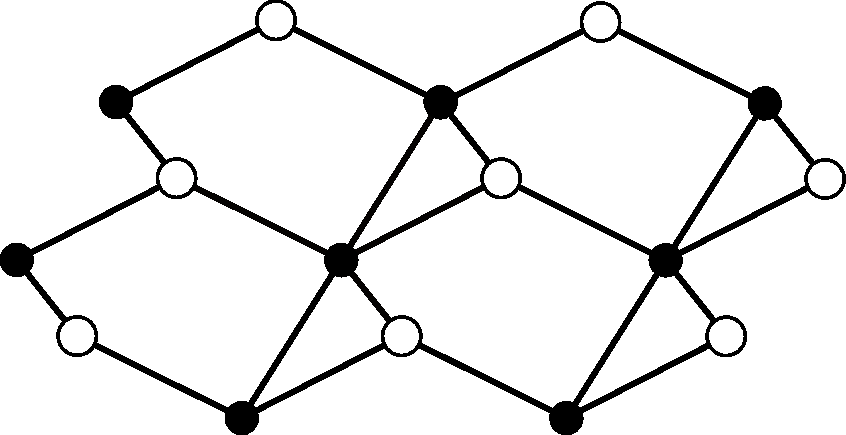
\includegraphics[height=3cm]{../figures/topologicalkeys.pdf}
%
%	Un filet (4 mailles représentées)
%\end{minipage}%
\begin{minipage}[t]{0.55\textwidth}
	\centering
	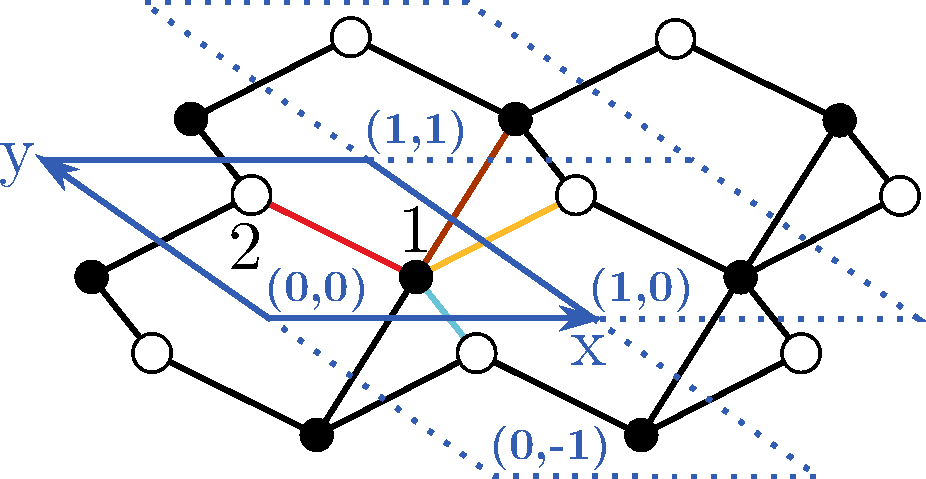
\includegraphics[height=4.5cm]{../figures/topologicalkeys2.pdf}
	
	Un graphe $2$-périodique avec une maille élémentaire en bleu et une numérotation des atomes.
\end{minipage}%
\begin{minipage}[t]{0.45\textwidth}
	\centering
	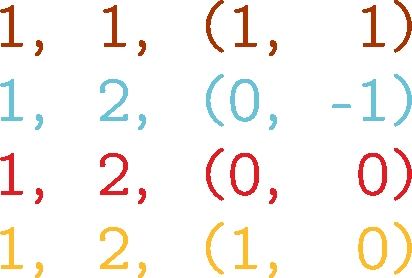
\includegraphics[height=3cm]{../figures/topologicalkeys3.pdf}

	La série d'arêtes directes correspondant à la représentation précédente.
\end{minipage}

\begin{enumerate}
	\item Écrire un type \jl{PeriodicGraph{N}} qui représente un tel graphe \jl{N}-périodique.
	
	\item Dans un graphe non-orienté, à chaque arête \textbf{directe} correspond une arête inverse, ou indirecte, qui lui est équivalente. Dans le cas des graphes périodiques, une arête directe est de la forme $(s, d, o)\in E$ avec soit  [$s < d$], soit [$s = d$ et le premier élément non-nul de $o$ est strictement positif]. Par exemple, l'arête $(1, 2, (0, -1))$ est directe car $1 < 2$, et l'arête indirecte associée est $(2, 1, (0, 1))$.

	Écrire une fonction \jl{edges(g::PeriodicGraph)} qui renvoie la liste des arêtes directes d'un graphe périodique.

	\item Un sommet d'un tel graphe périodique est représenté par une paire \jl{(i, ofs)} où $\jl{i}\in V$ est l'identifiant du sommet dans la maille élémentaire, et $\jl{ofs}\in\Z^N$ est la position de la maille dans laquelle se trouve le sommet. Par exemple, le sommet blanc lié par une arête cyan au sommet 1 de l'exemple est le sommet \jl{(2, (0,-1))}.

	Écrire une fonction \jl{neighbors(g::PeriodicGraph, x)} qui renvoie la liste des voisins du sommet \jl{x} dans le graphe \jl{g}.

	\textsl{Par exemple, si \jl{g} désigne le graphe de l'exemple, alors le sommet \jl{(1, (0,0))} doit se retrouver dans la liste renvoyée par \jl{neighbors(g, (2, (0,-1)))}, et inversement \jl{(2, (0,-1))} dans la liste des voisins de \jl{(1, (0,0))}.}
	
	\item La distance entre deux sommets d'un graphe non pondéré est le plus petit nombre d'arêtes qui permettent de relier ces deux sommets. Par exemple, un sommet est à distance 0 de lui-même et à distance 1 de tous ses voisins.

	La séquence de coordination d'un sommet $s$ dans un graphe périodique est la suite $\seq ui{\N^*}$ où pour tout $i\in\N^*$, $u_i$ est le nombre de sommets à distance $i$ de $s$.
	
	Écrire une fonction \jl{coordination_sequence(g::PeriodicGraph, s, dmax)} qui renvoie la séquence de coordination de \jl{s} dans \jl{g} jusqu'à la distance \jl{dmax}.
	
	\textit{Dans l'exemple, la séquence de coordination du sommet 1 attendue est $\paren{5\times i}_{i \in\N^*}$.}
\end{enumerate}

\end{document}